% !TEX encoding = UTF-8 Unicode

\documentclass[a4paper]{article}

\usepackage{color}
\usepackage{url}
%\usepackage[T2A]{fontenc} % enable Cyrillic fonts
\usepackage[utf8]{inputenc} % make weird characters work

\usepackage{graphicx}
\graphicspath{{../images/}}


\usepackage{courier}

\usepackage{enumitem}

\usepackage{color}

\definecolor{mygreen}{rgb}{0,0.6,0}
\definecolor{mygray}{rgb}{0.5,0.5,0.5}
\definecolor{mymauve}{rgb}{0.58,0,0.82}

\usepackage{fancyvrb}
\newcommand{\eng}[1]{(engl. \textit{#1})}
\newcommand{\zMQ}[0]{\textit{ØMQ}}

\usepackage{listings}
\lstdefinestyle{customc}{
  belowcaptionskip=1\baselineskip,
  breaklines=true,
  frame=L,
  xleftmargin=\parindent,
  language=C,
  šowstringspaces=false,
  basicstyle=\footnotesize\ttfamily,
  keywordstyle=\bfseries\color{green!40!black},
  commentstyle=\itšape\color{purple!40!black},
  identifierstyle=\color{blue},
  stringstyle=\color{orange},
}



\usepackage{parcolumns}





\usepackage[english,serbian]{babel}
%\usepackage[english,serbianc]{babel} %ukljuciti babel sa ovim opcijama, umesto gornjim, ukoliko se koristi cirilica

\usepackage[unicode]{hyperref}
\hypersetup{colorlinks,citecolor=green,filecolor=green,linkcolor=blue,urlcolor=blue}

%\newtheorem{primer}{Пример}[section] %ćirilični primer
\newtheorem{primer}{Primer}[section]

\begin{document}

\title{C++ Jezgro za Jupyter Notebook\\ \small{Seminarski rad u okviru kursa\\Metodologija stručnog i naučnog rada\\ Matematički fakultet}}

\author{Goran Vinterhalter, Marko Ranković \\ gvinterhalter@gmail.com, marko.rankovic@outlook.com}
\date{14.~april 2016.}
\maketitle

\abstract{
  C++ Jezgro pretstavlja softver koji pokušava da emulira interpretiranje c++
  tehnikama dinamičkog učitavanja pa izvršavanja. Zapravo funkcioniše kao
  shell za C++ ali može biti korišćen kao jezgro koje izvršava zahteve
  web aplikacij Jupyter Notebook.


\tableofcontents

\newpage

\section{Uvod}
\label{sec:uvod}


Jupyter Notebook je web aplikacija za kreiranje i deljenje dokumenata
koji pored uobičajenog tekstualnog sadržaja sadrže i interaktivni kod. 
\cite{Jupyter}

Dokument je sačinjen iz niza ćelija koje vizuelno mogu biti podeljene na ćelije običnog teksta (markdown)
i ćelije koda. Tokom izvršavanja, ćelijama koda biće pridružene ćelije sa rezultatima.
Dokumenti se čuvaju u JSON formatu a prikazuju se unutar web pregledača.
Na slici \ref{fig:nbPrimer} možemo videti primer notebook fajla u JSON obliku i prikaza u web pregledaču.

\begin{figure}[h!]
\begin{center}
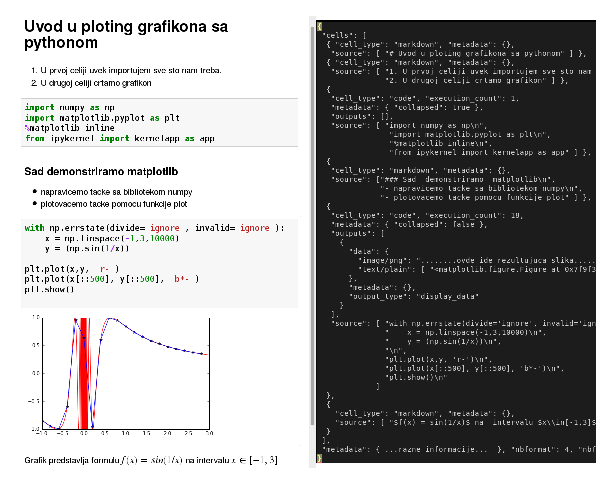
\includegraphics[scale=1]{nbPrimer}
\end{center}
\caption{Notebook primer}
\label{fig:nbPrimer}
\end{figure}

\section{Arhitektura}

Arhitektura softvera je server/klijent. \cite{IPython}
Serverski deo je sačinjen iz dve komponente kao što se da videti na slici \ref{fig:Kli-Serv}.
~\cite{IPython}

\begin{figure}[h!]
\begin{center}
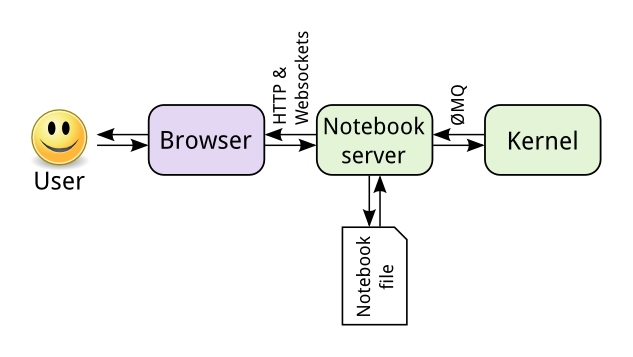
\includegraphics[scale=0.5]{nbKomponente.png}
\end{center}
\caption{Klijent Server arhitektura}
\label{fig:Kli-Serv}
\end{figure}

\begin{enumerate}
  \item Notebook server komunicira sa web pregledačem i dozvoljava kreiranje, gledanje i editovanje ćelija običnog teksta.
  \item Jezgro \eng{Kernel} je proces koji kao ulaz prima ćelije koda a vraća evaluiran izlaz. Pored toga Jezgro je takođe  zaduženo za stvari
    kao što su: samoispitivanje \eng{introspection}, dovršavanje koda \eng{code completition}, dokumentacija itd.
\end{enumerate}

Jezgro je prilagođeno za specifičan jezik. Recimo IPython jezgro izvršava python kod dok postoje i:
IJulia, IRuby, IHaskell, IJavaScript, IRKernel i mnogi drugi.
Cilj ovog seminarskog rada je da izuči mogućnosti pravljenje jezgra za jezik c++ i izradi prototipa.
Na prvi pogled problem deluje trivijalan, ćelije se kompajliraju i izvršavaju, ali nije baš tako.

Jupyter notebook se inicijalno zvao IPython notebook i razvio se iz IPython projekta koji pretstavlja front end za
python interpreter. Primarni cilj Ipython notebook projekta je bio interaktivna platforma u kojoj
bi korisnik u jednoj ćeliji mogao da izvrši definisanje recimo promenljive ili funkcije a da je koristi u nekoj drugoj ćeliji.
Takav pristup idelano odgovara jezicima koji se interpretiraju što C++ nije.
Posle nekog vremena se shvatilo da je notebook pristup primenljiv i na druge interaktivne jezike pa je
projekat preimenovan u Jupyter Notebook za koga se razvijaju različita jezgra (oficijalno samo IPython).
Ali kako napraviti C++ Jezgro?

Trivijalni pristup bi bio da Jezgro za C++ čuva sve definicije i da ih aranžira u jedan veliki fajl koji bi svaki
put morao da bude kompajliran pa izvršen. Ovakav pristup ima mane:

\begin{itemize}
    \item Kompilacija nepotrebno velikih fajlova je skupa.
    \item 
      Česta je potreba da korisnik u prvim ćelijama izvrši neku skupu
      operacije, recimo učita i obradi neku veliku datoteku.
      Ako bi se sve čuvalo u jednom fajlu koji bi se konstantno
      ponovo ceo izvršavao onda bi se svaki put ta velika datoteka morala ponovo obrađivati.

    \item Ne pretstavlja bas interaktivan pristup radu.
\end{itemize}

Jedinu dužnost koju  Jezgro ima jeste komunikacija sa Notebook serverom preko \eng{ ØMQ (a.k.a ZeroMQ)}.
Dakle Jezgro može da bude implementiran u bilo kom jeziku i da bude sačinjen iz jednog ili više procesa
koji opet mogu biti implementirani u jednom ili više programskih jezika. 

Pošto je ovaj projekat implementiran u jeziku python i već postoji klasa \eng{ipyKernel.kernelbase.Kernel}
koja se može naslediti zarad pravljenja jednostavnog omotača koji implementira \zMQ  komunikaciju odlučili
smo se da prototip implementiramo na taj način. \cite{IPython}

U ostatku teksta fokusiraćemo se na primenu dinamičkog učitavanja \eng{dynamic loading} za simuliranje
interaktivnog rada sa C++ jezikom ali prvo treba detaljnije opisati protokol za poruke \eng{Message protocol}
koji takođe specifikuje zaduženja jednog Jezgra.



\section{Protokol za poruke}
\label{sec:Poruke}

Bitno je istaći da jedno jezgro može biti konektovano na više klijenata \eng{font end's} \cite{IPython}

Jezgro treba da implementira 4 soketa \eng{socket} (prva 3 su bitna): \cite{Ipython}
\begin {enumerate}
\item \textbf{Shell} - \eng{single Router} soket, koji podržava konekcije ka nekoliko
  klijenata. Namenjen je za zahteve izvršavanja koda, ispitivanje objekata itd.

\item \textbf{IOPub} - takozvani  \eng{broadcast channel} koji služi za sve sporedne
  efekte tipa: stdout, stderr.

\item \textbf{stdin} - Ovaj ruter soket je povezan na sve klijente i služi da
  jezgro zatraži ulaz od korisnika klijenta.

\item \textbf{Control} - Isto kao i \textbf{Shell} ali služi za abort, shutdown i
  druge bitne zahteve koji ne treba da čekaju u redu da se pošalju kroz \textbf{Shell}.
\end {enumerate}


\subsection{Struktura i tipovi poruka}
\label{sec:Pformat}

Trenutno poruke se šalju u \eng{JSON} formatu a u pythonu se pretstvaljaju 
Rečnikom rečnika prikazanim u \ref{fig:struktPoruka} \cite{IPython}

\cite{IPython}

\begin{figure}[h!]
\begin{center}
  \begin{verbatim}
{
  'header' :{
    'msg' : uuid,
    'username' : str,
    'session' : uuid,
    'msg_type' : str,
    'version' : 5.0
  }

  'parent_header' : dict,
  'metadata' : dict,
  'content' : dict
}
\end{verbatim}
\end{center}
\caption{Struktura poruke}
\label{fig:struktPoruka}
\end{figure}

Nećemo ulaziti u detalje implementacije komunikacije preko \zMQ jer korišćenjem
\eng{ipyKernel.kernelbase.Kernel} klase dobijamo već gotovu osnovu jezgra.
Pomenutoj klasi je dovoljno premostiti \eng{override} pretefinisane funkcije
koje kao povratnu vrednost prosleđuju rečnik koji odgovara povratnoj poruci. \cite{Ipython}

Da bi razumeli ponašanje, ulaz i izlaz funkcije koje treba implementirati
moramo da znamo koje poruke pristižu i kako odgovoriti na njih.
Mi ćemo razmotiti samo par bitnih poruka a željne čitaoca upućujemo na 
detaljnu dokumentaciju svih poruka: \\
\url{www.jupyter-client.readthedocs.io/en/latest/messaging.html#messages-on-the-shell-router-dealer-sockets}


\subsection{Tipovi poruke}
\label{sec:PTipPoruke}


Poruka \eng{execute\_result} \ref{fig:execute} je obrađena python funkcijom \eng{do\_execute}. \\
Ovo je najbitnija funkcija za jezgro jer kao ulaz prima kod koji treba izvršiti a kao izlaz vraća rezultat.


\begin{figure}[h!]
\begin{center}

  \begin{verbatim}
execute_request = {
  'code': str,      #kod koji treba izvršiti
  'silent': bool,   #da li se uvećava brojač i ispisuje rezultat
  'store_history': bool, # ne ako je silent = True
  'user_expressions': dict,
  'allow_stdin': True,
  'stop_on_error': False,
}      
\end{verbatim}
\end{center} 
\caption{Poruka \eng{execute\_request}}
\label{fig:execute}
\end{figure}

status rezultata može biti: 'ok', 'error' ili 'abort'. 
Odgovor sadrži status, broj izvršavanja engl{execution\_count} a zavisno od tipa
statusa dodaju se dodatna polja koja možemo videti na prikazu \ref{fig:execute_reply}


\begin{figure}[h!]
\begin{center}

\begin{verbatim}
execute_reply = {
  'status': = 'abort'
  'execution_count' : int
  # nema dalje
}      

execute_reply = {
  'status': = 'error'
  'execution_count' : int

  'payload' : list(dict), # deprecated
  'user_expressions' : dict,
}      

execute_reply = {
  'status': = 'error'
  'execution_count' : int

  'ename' : str    # ime greške
  'evalue': str    # vrednsot greške
  'traceback' list  #  trag izvršavanja
}      
\end{verbatim}
\end{center} 
\caption{Poruka \eng{execute\_reply}}
\label{fig:execute_reply}
\end{figure}


Nabrajamo još neke bitne poruke

\input{../Poruke.tex}





\section{Rad Jezgra}
\label{sec:Jezgro}

Da bi opisli rad i implementaciju jezgra uzećemo jednostavan primer.
Pretpostavimo da je korisnik kreirao tri ćelije.
Ćelije su numerisane i izvršavaju se zadatim redosledom.
U realnosti jezgro ne zna koja ćelija je koja. 
On samo dobija  kod koji treba da izvrši kao gore pomenuti execute\_request a
numeracija služi nama da olakša primer.

\begin{enumerate}

\item 
\begin{verbatim}
#include <iostream>
using namespace std;
int a = 2;
string b = "Hello";
%r cout << a << " "; //%r je magic, opisacemo kasnije
%r cout << b << endl;
void f(int i, string & s){
  while(i--)
    cout << i << ": "<<  << s << " ";
}
\end{verbatim}


\item 
\begin{verbatim}
void g(void){
  f(a, b);
}
\end{verbatim}


\item 
\begin{verbatim}
%r g(a, b);
%r a = 5;
%r g(a, "World");
\end{verbatim}

\end{enumerate}


Implementacija izvršavanja svake od tri ćelije se sastoji od 3 dela:
\begin{enumerate}
  \item kompajliranje - Ćelija se prevodi u deljeni obejkat \eng{shared object, .so}
    koji je \eng{position independent}
  \item dinamičko učitavanje \eng{dynamic loading} - jezgro dinamički učitava .so pri čemu se
    linker razrešava sve extern simbole. Biće reči o ovome kasnije.
\item izvršavanje - ćelija se izvršava. Naša implementacija radi tako što svaki deljeni objekat potencijalno
  ime funkciju 'run' koja ako postoji biva pozvana nakon učitavanja.
\end{enumerate}

Da bi se kod uspešno izvršio svaka od ćelija se obrađuje na sledeći način:

\begin{enumerate}
    \item Uklanjamo komentare iz koda ("nije neophodno ali čini \eng{ad hoc} parsiranje lakšim")
    \item Razrešuju se takozvane magične \eng{magic} naredbe. To su naredbe koje
      počinju sa '\%' ili '\%\%'. O tome više reči kasnije
    \item Parsira se prosleđeni izvorni kod i izvlače informacije:
      \begin{itemize}
          \item globalni simboli koji se definišu u kodu. (promenljive i funkcije, za sada)
          \item deklaracije tipova
          \item definicije makroa
          \item using direktive
          \item include naredbe
      \end{itemize}
      Ovo informacije se čuvaju jer će biti potrebne za narednu ćeliju koja se bude izvršavala,
      verovatno će referisati na nešto što je ova ćelija deklarisala.
    \item Sav kod koji ne čini deklaracije i definicije već izraze koje treba evaluirati
      moramo nekako da razlikujemo od ostatka koda. U našoj implementaciji odabrali smo
      jednoliniski magiju '\%r' da bude prefiks za ovakav izraze.
      (izraz mora da bude jednoliniski). Ako '\%r' postoji onda će na kraju koda
      biti dodata funkcija 'void \_\_run\_\_(void) { ...  }' koja će sadržati sve
      pomenute izraze.
    \item Da bi kod uspešno prošao kompilaciju moraju se dodati deklaracije
      svih refereisanih simbola, include i ostale direktive koje su bile korišćen
      pri izvršavanju pređašnjih ćelija. Bilo bi idealno dodati samo ono što treba
      ali to je komplikovano izvesti zato dodajemo sve. Izuzetak su simboli
      koji imaju novu deklaraciju u smislu da im se menja tip.

\end{enumerate}

Treba primetiti da se svaki prosleđen kod razvrstava na delove sa definicijama
i delove sa izrazima koje treba izvršiti. Kako kompilacija i učitavanje 
definicija simbola ide prvo, kod koji naizmenično ima defincije i izraze nije moguće
korektno prevesti na ovaj način. Međutim često je programerska praksa da 
se prvo navedu sve definicije. Ovo bi se naravno moglo popraviti. Recimo
da se svaki izraz ćelije kompajlira pa izvršava, ali to pravi nepotrebnu kompleksnost
i nećemo razmatrati takvo rešenje. 

Naš primer sa tri ćelije bi bio obrađen ovako:

\begin{enumerate}
    \item Prva 
      
    \begin{verbatim}
#include <iostream>
using namespace std;
int a = 2;
string b  = "Hello";
void f(int i, const string & s){
  while(i--)
    cout << i << ": " << s << " ";
}
void __run__(void) {
cout << a;
cout << b << endl;
}
-------------
izlaz:
2Hello
      \end{verbatim}

  \item Druga ćelija sadrži samo jednu funkciju ali referiše globalne simbole

      \begin{verbatim}
#include <iostream>
using namespace std;
extern string b  ;
extern int a ;
void f(int i, const string & s);

void g(void){
  f(a, b);
}
  ----------
      \end{verbatim}

  \item Treća ćelija sadrži samo izraz koji treba evaluirati

      \begin{verbatim}
#include <iostream>
using namespace std;

extern string b  ;
extern int a ;
void f(int i, const string & s);
void g(void);

void __run__(void) { 
  g();
  a = 5;
  f(a, "World"); 
}
  ----------
izlaz:
1: Hello 0: Hello 4: World 3: World 2: World 1: World 0: World
      \end{verbatim}

\end{enumerate}

Svako izvršavanje koda,  može potencijalno
da izazove bacanje nekog izuzetka ili signala tipa segmentation fault. Jezgro
ne bi smelo da bude ugašeno u slučaju pojave ovakvog tipa greške.
Izvršavanje koda i učitavanje onda treba ili raditi u nekom drugom procesu ili bi
se više pažnje trebalo posvetiti baratanju izuzecima i signalima.

Još jedan razlog zašto bi izvršavanje trebalo da bude zaseban proces je
kad se traži ulaz od korisnika. Proces koji se izvršava može da zalagvi dok
jezgro traži ulaz od korisnika.

Naša implementacija nažalost sve obavlja u jednom procesu te stoga i nema mogućnost
da korektno obradi potražnju ulaza od korisnika.


\subsection{Magije}

Ipython je uveo pojam magije \eng{magic} kao komande specijalno značenja za
proširenje mogućnosti python jezika. IPython jezgro razlikuje: \cite{magic}
\begin{enumerate}
  \item liniske (\%komanda) 
    recimo \%ls printa sadržaj direktorijum, dok \%time 'python-komanda'
    računa srednje vreme izračunavanje 'python-komande'
  \item ćeliske (\%\%komanda) 
    magija se odnosi na celu ćeliju. Recimo moguće je izvršiti neki jezik koji nije python
    \%\%latex ... označava da će ćelija biti obrađena kroz latex
\end{enumerate}

Mi definisemo linisku magiju '\%r' koja označava linije koda koje treba izvršiti po ucitavanju.
Liniske magije su implementirane kao inekcije c++ koda  a ćeliske magije
imaju proizvoljnu implementaciju.



\subsection{Dinamičko učitavanje}
\label{sec:dUcitavanje}

Dinamičko učitavanje (Dynamic loading) je mehanizam  da se procesu koji se izvršava
učitaju dodatne funkcije, klase itd iz neke biblioteke tj.
deljene datoteke \eng{shared object, .so} 
\cite{LinkersAndLoaders}. Najčešća uloga kod kompleksnijih aplikacija
jeste proširivanje funkcionalnosti preko takozvanih proširenja \eng{plugin}.
Svaki plugin se kompajlira u zasebni deljeni obejkat koji po potrebi biva učitan u glavnu aplikaciju.


Postoji C biblioteka dlfcn koja definiše funkcije za dinamičko učitavanje (dlopen, dlclose, ...)
Takođe Python modul ctypes pored drugih stvari pruža i interfejs ka ovoj biblioteci i znatno
pojednostavljuje proces.  \cite{dlopen}

\noindent\begin{minipage}[t]{.45\textwidth} \begin{verbatim}
in.so
==============
extern "C" {
  int a = 25;
  string b = "Hello World";
  vector<int> lista= {1,2,3,4};
  void print(){
    cout << ", "  << b
    << ", " << lista << endl;
  }
}
\end{verbatim} \end{minipage}\hfill
\begin{minipage}[t]{.45\textwidth} \begin{verbatim}
in1.so
==============
extern "C" {
  extern int a;
  void print();

  void f(){
    a = 100;
    print();
  }
}
\end{verbatim} \end{minipage}


Učitavanje u pythonu

\begin{verbatim}
from ctypes import *                                                            
prog = CDLL('./in.so', mode=RTLD_GLOBAL|RTLD_DEEPBIND|RTLD_NOW)                                        
prog.print()                                                                    
prog1 = CDLL('./in1.so', mode=RTLD_GLOBAL|RTLD_DEEPBIND|RTLD_NOW)                                      
prog1.f() 
\end{verbatim}

Bitno je uočiti da f() referiše simbole iz prvog in.so deljenog objekta.
ctypes niti dlopen ne pružaju mogućnosti samoispitivanja deljenog objekta.
Mi moramo da znamo kakve simobole deljeni objekat sadrži.
Zato smo gore odabrali da uvek imamo jednu funkciju istog imena \_\_run\_\_.

\begin{itemize}
  \item RTLD\_GLOBAL - govori da će svi učitani simboli biti globalno vidljivi za razrešavanje i \cite{dlopen}
    pri sledećem učitavanju. To nam je neophodno.
  \item RTLD\_DEEPBIND - govori da će simboli prvo biti traženi u deljenoj datoteci koja se učitava \cite{dlopen}
  \item RTLD\_NOW - govori da će svi simboli biti rešeni pri učitvanju (RTLD\_LAZY suprotan flag) \cite{dlopen}
\end{itemize}

poslednje 3 pomenute opcije nisu definisane u python modulu ctypes. Moraju se dodefinisati.
RTLD\_DEEPBIND nije specifikovan u POSIX.1-2001

Zanimljivo  pitanje koje se nameće jeste. A šta ako u primeru sa 3 ćelije izvršimo
još jednu sa kodom 

\begin{verbatim}
long a = 10;
%r cout << a;
\end{verbatim}

Dobili bi očekivan izlaz "10".

Međutim ako bi opet u petoj ćeliji pokrenuli "\%r cout << a;" dobili bi
ponovo "5". To je zato što je u četvrtoj ćeliji DEEPBIND garantovao da će
biti nađen verzija sa long dok u petoj ćeliji pretraga za definicijom 'a'
ide linearno i prvo nailazi na deklaraciju sa int. Sve što bi trebalo uraditi
jeste pretragu izvršavati od poslednje učitane datoteke do prve ali trenutno
ne znamo kako to da izvedemo.

\subsection{Parsiranje}
\label{sec:pars}

Parsiranje C++ izvornog koda je najteži korak.
Trenutna implementacija koristi ctags i regularne izrze za od hoc parsiranje.
Ovo svakako nije dobra praksa i ubuduće zahteva ozbiljne popravke.

Jedno rešenje je korišćenje biblioteka clang kompajlera.
Clang za ovu svrhu nudi dve biblioteke. Lakša je C biblioteka libclang i za nju
postoji python binding. \cite{Clang}

Ispod dajemo kratak primer koji prikazuje parsiranje jednog cpp fajla.
Ne ispisujemo sve čvorove apstraktnog stabla parsiranja jer nisu potrebni.
Nažalost još nismo sigurni kako da dobijem sve informacije koje su nam potrebne.

\noindent\begin{minipage}[t]{.45\textwidth} \begin{verbatim}
test.cpp
===========
#include <stdio.h>
int a = 42;
float b= 3;
int * p, & nop(a), x;

int f(){
  int c = 4 + b;
  return a + c;
}
struct Vec{
  int x, y;
};
float g(int a, int b){
  return a*b;
}
static char c = 'x';
int main(){
  return 0;
}
        \end{verbatim} \end{minipage}\hfill
        \begin{minipage}[t]{.45\textwidth} \begin{verbatim}
parsing test.cpp
============
test.cpp (TRANSLATION_UNIT) :  
  a (VAR_DECL) :  int a = 42 ;
     (INTEGER_LITERAL) :  
  b (VAR_DECL) :  float b = 3 ;
     (UNEXPOSED_EXPR) :  
       (INTEGER_LITERAL) :  
  p (VAR_DECL) :  int * p ,
  nop (VAR_DECL) :  int * p , & nop ( a )
    a (DECL_REF_EXPR) :  
  x (VAR_DECL) :  int * p , & nop ( a ) , x ;
  f() (FUNCTION_DECL) :  int f ( ) { int c = 4 + b ; return a + c ; } struct
  Vec (STRUCT_DECL) :  struct Vec { int x , y ; } ;
    x (FIELD_DECL) :  int x ,
    y (FIELD_DECL) :  int x , y ;
  g(int, int) (FUNCTION_DECL) :  float g ( int a , int b ) { return a * b ; } static
    a (PARM_DECL) :  int a ,
    b (PARM_DECL) :  int b )
  c (VAR_DECL) :  static char c = 'x' ;
     (CHARACTER_LITERAL) :  
  main() (FUNCTION_DECL) :  int main ( ) { return 0 ; }
        \end{verbatim} \end{minipage}

python binding za libclang ne pokriva sve mogućnosti biblioteke ali
se zato to može lako dodati. Veći probelm je što sama biblioteka libclang
iako stabilna ne pruža finu kontrolu nad generisanim apstraktnim stablom.


\section{Zaključak}
\label{sec:zakljucak}

U ovom radu pretstavili smo softver Jupyter Notebook i istražili smo mogućnosti
razvoja Jezgra za C++ jezik koji bi izvršavao c++ kod.
Pokazali smo da je tehnikom dinamičkog učitavanja moguće donekle simulirati
interpretaciju ali i dalje postoje male razlike koje bi trebalo rešiti.
Implementacija pravog Jezgra bi se mnogo više oslanjala na libclang biblioteku.
U našim razmatranjima libclang je korisna za parsiranje ali postoje i mnoge druge
dužnosti Jezgra kao što je samoispitivanje objekata, dovršavanje koda itd.

\addcontentsline{toc}{section}{Literatura}
\appendix
\bibliography{../seminarski} 
\bibliographystyle{plain}

% \appendix
% \section{Dodatak}


\end{document}


